\RequirePackage{amsmath}
\documentclass{llncs}

\usepackage[caption=false]{subfig}
\usepackage{graphicx}
\usepackage{bm}
\usepackage{float}
\usepackage{amssymb}
\usepackage{moreverb}
\usepackage{color}
\usepackage{amsmath}
\usepackage{color}
\usepackage{url}
\usepackage{bbding}
\usepackage{booktabs}
\usepackage[numbers]{natbib}

%
\begin{document}
\title{On Exploring Hidden Structures Behind\\ Cervical Cancer Incidence}
%\titlerunning{}
\author{Niko Lietz\'{e}n \inst{1}\thanks{Work of N. Lietz\'{e}n was supported by Emil Aaltonen Foundation (grant 170156 N).}  \and Janne Pitk{\"a}niemi \inst{2,3} \and Sirpa Hein{\"a}vaara \inst{2} \and Pauliina Ilmonen \inst{1}}



\institute{Department of Mathematics and Systems Analysis, Aalto University School of Science, Helsinki, Finland, \email{\{niko.lietzen, pauliina.ilmonen\}@aalto.fi} \and Institute for Statistical and Epidemiological Cancer Research, Finnish Cancer Registry, Helsinki, Finland,  \email{\{janne.pitkaniemi, sirpa.heinavaara\}@cancer.fi} \and Department of Public Health, University of Helsinki,  Finland }


\maketitle




\begin{abstract}
Finding novel latent structures in time related variation in disease incidence  may reveal new etiological components and is of great interest in disease  epidemiology. We introduce  time series version of invariant coordinate selection (tICS) as an exploratory tool in the search of hidden structures in the analysis of population-based registry data.  Increasing cancer burden inspired us to consider  a case study of age stratified cervical cancer incidence time series data in Finland between the years 1953 and 2014. The latent components, that we uncovered using tICS, support recent findings of calendar time varying contribution of early and late age related components in cervical cancer. 
Furthermore, we could explain most of the variation of cervical cancer incidence in different age groups by using only two latent tICS components. The second tICS component is particularly interesting, since it clusters the age groups according to the age of menopause. Our case study results imply that the etiology behind cervical cancer differs by age group. 
\end{abstract}

\section{Introduction}\label{intro}
Increasing cancer burden has made researchers worldwide search for factors that explain  trends in cancer incidence data \citep{parkin2011}. In addition to age, period, and cohort, several other observable factors have an effect on the trends in cancer incidence. Improved diagnostics, organized cancer screening programs, and general awareness have increased the  cancer incidence for many cancers. Additionally, some known lifestyle related factors have an effect on the cancer incidence. For example, changes in smoking prevalence have a clear delayed effect on the incidence of lung cancer. However, there are also unknown underlying factors that have effects on cancer incidence rates. Identification and quantification of those unknown factors would further help in understanding the trends in cancer incidence data.

In this paper, we consider a time series version of invariant coordinate selection (ICS) in the context of latent components of calendar time variation in incidence. ICS has been previously applied in numerous medical applications. It has been applied successfully to analyze e.g. EEG data sets of the brain \cite{joyce2004} and to cluster mammogram data sets \cite{gallardo2012}.
We use the transformation as an exploratory tool in search of hidden structures of cervical cancer incidence time
series data. The data set is from Finland between the years 1953 and 2014 and it is available online \cite{engholm2010}.

ICS is closely related to the more famous independent component analysis (ICA). Under some assumptions, the ICS procedure provides a solution to the independent component problem. The objective in ICS is to transform the observed data into an invariant coordinate system. Occasionally,  the new coordinate system reveals structure from the data that is not originally visible. The clear advantage of ICS when comparing to e.g. the frequently used principal component analysis (PCA) is that the chosen scales and units of measurement have no effect on the results. 

%The goal of this paper is to illustrate the time series version of ICS as a feasible  exploratory tool, compared to e.g. the commonly used PCA. }




\section{Invariant Coordinate Selection}\label{secpca}


In this section, we review the scatter matrix based invariant coordinate selection method introduced in \cite{TY}.


Let $X \in \mathbb{R}^{n\times p}$, where $n>p$. A location functional is a $p$-vector valued statistic $\hat{T}\left(X\right)$, that is affine equivariant in the sense that
\begin{align*}
\hat{T}\left(AX+b1_n^\top\right)=A\hat{T}\left(X\right)+b
\end{align*}
for all nonsingular $p\times p$ matrices $A$ and for all $p$ vectors
$b$.
Likewise, a  
positive definite $p\times p$ matrix valued statistic $\hat{S}\left(X\right)$ is a scatter matrix, that is affine
equivariant in the sense that
\begin{align*}
\hat{S}\left(AX+b1_n^\top\right)=A\hat{S}\left(X\right)A^\top
\end{align*}
for all nonsingular $p\times p$ matrices $A$ and for all $p$ vectors
$b$.



Elementary examples of a location functional and a scatter matrix are
the sample mean vector and the sample covariance matrix. There are several other location functionals and scatter matrices, even families of them, that have different desirable properties, e.g. robustness, efficiency, limiting multivariate normality and computational efficiency \cite{S3,S2,MMY}.





Let $\hat{T}_1\left(X\right)$ denote an arbitrary but fixed location functional, and let $\hat{S}_1\left(X\right)$ and $\hat{S}_2\left(X\right)$ denote  arbitrary but fixed and different scatter matrices. The invariant coordinate selection (ICS) transformation $\hat{\Gamma}\left(X\right)$ for the data $X$ is  defined such that if 
\begin{align*}
Z=\hat{\Gamma}\left(X\right)\left(X-\hat{T}_1\left(X\right)1_n^\top \right),
 \end{align*}
 then
\begin{align*}
\hat{T}_1\left(Z\right)=0, \  \hat{S}_1\left(Z\right)=I_p,  \ \mbox{and} \  \hat{S}_2\left(Z\right)=L=\textnormal{diag}\left(l_1, ..., l_p\right),
\end{align*}
where the diagonal elements of the diagonal matrix $L$ are in decreasing order.


If the data arises from a continuous distribution, then the transformation matrix $\hat{\Gamma}\left(X\right)$ is almost surely unique up to the signs of its row vectors. Consequently, it is affine equivariant up to the signs, and it can be used to transform the data to up to signs invariant coordinates. Thus, affine  transformations to the original data have no  effect on the procedure. The transformation ensures that when examining the transformed data, the findings are true findings and not artefacts of the chosen coordinate system. 
Note that whereas principal component analysis (PCA) makes data uncorrelated, ICS makes data independent with respect to two measures of linear dependence. ICS transformation can be seen as affine invariant PCA that, on top of first order dependencies, considers second order dependencies as well. Moreover, whereas PCA is highly affected by scaling of the variables,  ICS, due to affine invariance, is not affected by scaling at all.

It can be shown that if the chosen location and scatter estimates converge, so do the statistics $\hat{\Gamma}$ and $L.$ Moreover, under the assumption of asymptotic normality of the location and scatter estimates, the statistics $\hat{\Gamma}$ and $L$ are also asymptotically normal \cite{i4c,i4,i8}.

The scatter matrix based invariant coordinate selection transformation was first introduced in the context of independent component analysis (ICA) \cite{FOBI}. It was based on the use of the regular covariance matrix and the scatter matrix based on fourth moments. The transformation was named the fourth-order blind identification (FOBI) transformation. Later, the ICS transformation was considered in wider settings \cite{TY}. In the independent component model, the elements of a $p$ variate random vector are assumed to be linear combinations of the elements of an unobservable $p$ variate vector with mutually independent components. The aim in ICA is to recover the independent components by estimating an unmixing matrix that transforms the observed $p$ variate vector to  independent components \cite{IN}. Assuming that the chosen scatter functionals have the independence property, the ICS functional $\hat{\Gamma}$ provides a solution for the ICA problem \cite{FOBI,i4,Nordhausen:2008,Oja:2006}.  Under the assumption of i.i.d. observations, the use of the scatter matrix based ICS transformation has not  been limited to ICA. It has been applied in finding hidden underlying structures of data, in constructing affine invariant depth functions, in dimension reduction, in analysing mixture models, and in defining multivariate skewness and kurtosis measures \cite{i4c,i4,i8,Serfling2010,TY}.


For time series data, we can obtain transformations similar to ICS, by replacing the second scatter matrix in the transformation by an  autocovariance matrix.  Depending on the data set, we could also use two autocovariance matrices with different lags.  Autocovariance 
matrix based transformations have been applied to time series ICA in settings where the observations are
uncorrelated second order stationary time series \cite{Miettinen2012,Tong1990}.  In the context of second order stationary time series data, the procedure is called the algorithm for multiple unknown signals extraction (AMUSE) \cite{Tong1990}. Like the
scatter matrix based ICA was extended to ICS, we consider applying
AMUSE transformation in  wider settings.
We use it in dimension reduction and as an exploratory
tool in the search of hidden structures in our case study of cancer incidence time
series data. 

\section{Invariant Coordinate Selection for Time Series Data}\label{tics}
In this section, we consider autocovariance matrix based transformations that have previously been applied to uncorrelated second order stationary time series data \cite{Miettinen2012,Tong1990}.


Let $X\in \mathbb{R}^{n\times p}$ be a $p$-variate discrete times series that contains $n$ observations and denote the $i$th row of $X$ by $x_i$. Furthermore, let $\tau \in \left\{0,1,\ldots,n-1\right\}$ and let $\hat{T}\left(X\right), \hat{S}_0\left(X\right),$ and $\hat{S}_{\tau}\left(X\right)$ denote the sample mean vector, the sample covariance matrix, and the sample autocovariance matrix with lag $\tau$, respectively, that are computed from the data $X.$ The sample autocovariance matrix is defined as 
\begin{align*}
\hat{S}_{\tau}\left(X\right)=\frac{1}{\left(n -\tau\right)} \sum^{n-\tau}_{j=1}\left(\left(x_j - \hat{T}\left(X\right)\right)\left(x_{j+\tau} - \hat{T}\left(X\right)\right)^\top \right),
\end{align*}
where the sample covariance matrix is obtained with $\tau=0$, up to a constant. 

Note that $\hat{S}_\tau$ does not necessarily produce symmetric estimates. The symmetrized version of the autocovariance matrix is obtained by
\begin{align*}
\hat{S}_\tau^\textnormal{S} = \frac{1}{2} \left( \hat{S}_\tau + \hat{S}^\top_\tau \right),
\end{align*}
which is a more convenient estimator since the population quantities of scatter are usually assumed to be symmetric.

 The time series invariant coordinate selection transformation matrix, i.e. the unmixing matrix, $\hat{\Gamma}\left(X\right)$ for the data $X$ is now defined such that if 
\begin{align*}
Z= \hat{\Gamma}\left(X\right)\left(X-\hat{T}\left(X\right)1_n^\top\right),
\end{align*}
then
\begin{eqnarray*}
\hat{T}\left(Z\right)=0\text{ } \text{ , } \text{ }  \  \hat{S}_0\left(Z\right)=I_p  \text{ } \text{ and } \text{ }  \hat{S}^\textnormal{S}_{\tau}\left(Z\right)=\Lambda=\text{diag}\left(\lambda_1, ..., \lambda_p\right),
\end{eqnarray*}
where $|\lambda_1|\ge ...\ge |\lambda_p|>0$.



For general time series data, we call the transformation time series ICS or shortly tICS. The tICS transformation transforms time series data to invariant coordinates and it may be used in dimension reduction and/or as an exploratory tool in the search of hidden structures from time series data. We can think that ICS is an extension to PCA and tICS is incorporating the time series structure to the ICS transformation.

The efficiency of the tICS procedure depends strongly on the choice of the parameter $\tau$. The approach proposed in literature is to try different values of $\tau$ and  choose the parameter such that the estimate $\Lambda$ has as distinct diagonal elements as possible  \cite{amari2002}.


Note that,
\begin{align*}
\hat{S}_0\left(X\right)^{-1}\hat{S}_{\tau}^\textnormal{S}\left(X\right) \hat{\Gamma}\left(X\right)^\top =\hat{\Gamma}\left(X\right)^\top\Lambda,
\end{align*}
i.e. like in the case of regular ICS, the diagonal elements of $\Lambda$ are the eigenvalues of $\hat{S}_0\left(X\right)^{-1}\hat{S}^\textnormal{S}_{\tau}\left(X\right),$ and the column vectors of $\hat{\Gamma}\left(X\right)^\top$ are the corresponding eigenvectors. And again, if the diagonal elements of $\Lambda$ are distinct, then the solution is unique up to the signs of the eigenvectors.
If the data arises from a continuous distribution, then the transformation matrix $\hat{\Gamma}\left(X\right)$ is almost surely unique up to the signs of its row vectors. Consequently, it is affine equivariant up to the signs, and it can be used to transform time series data to invariant coordinates.

After deriving the estimate $\hat{\Gamma}\left(X\right) = \hat{\Gamma}\in \mathbb{R}^{p\times p}$,  the observed centered curves can be  estimated using the inverse $\hat{\Gamma}^{-1}$ such that
\begin{align}
\label{estimation}
\hat{x}_t\left(i\right)= \sum_{k=1}^q  \left[\hat{\Gamma}^{-1}\right]_{ik} z_t\left(k\right) , \ t\in {1, ...., n}
\end{align}
where $i \in \left\{1,\ldots p\right\}$ is the $i$th column of $X$, $q$ is the number of underlying components we  use to estimate the original time series, $z_t\left(k\right),$ $k \in \left\{1,\ldots p\right\}$, is the $k$th column of the transformed data, i.e. the $k$:th estimated tICS component at time point $t$, and $\hat{x}_t\left(i\right)$ is the resulting estimate of the observed $i$th time series at a point of time $t$. Note that if we use all the tICS components, i.e. choose $q=p$, the estimates are then exactly the centered version of the original time series.



\section{Underlying Trends in Cancer Incidence}\label{data}
In this section, we apply time series ICS transformation to time series data of age stratified cervical cancer incidence rates between years 1953 and 2014 in Finland.
These long-term cervical cancer data from 1953--2014 in Finland were obtained from the population-based cancer registry with excellent quality and coverage of registration of solid tumors \cite{leinonen2016,teppo1994}. The data is available on  the web page of the NORDCAN project \cite{engholm2010}.

During this 60--year period, cervical cancer incidence has been affected mostly by the nationwide screening program \cite{hakama1975}. The organized cervical cancer screening program was introduced in 1963 and it reached full coverage in the early 70s. Screening invitations are sent to females between 30 and 60 years of age in every five years. In some municipalities, invitations are extended also to females aged 25 and/or 65 years. Thus, we have divided the data into five year age groups.  There have been clear changes, mostly in the years and the age groups subject to organized screening. We  search for underlying structures that can be used in describing other changes in cancer incidences over the years. 
 
 The age groups of younger than 35 have been combined  into a single group. Likewise, age groups of older than 74 have been combined into a single group. Thus, our data set contains 10 separate age groups, resulting in a 10 dimensional time series with 62 observations. Annual incidences of the different age groups  are  presented in Fig. \ref{p1b}. Furthermore, the sample mean time series of the cervical cancer incidence is presented as a black curve in Fig. \ref{p1b}.
\begin{figure}
   \centering
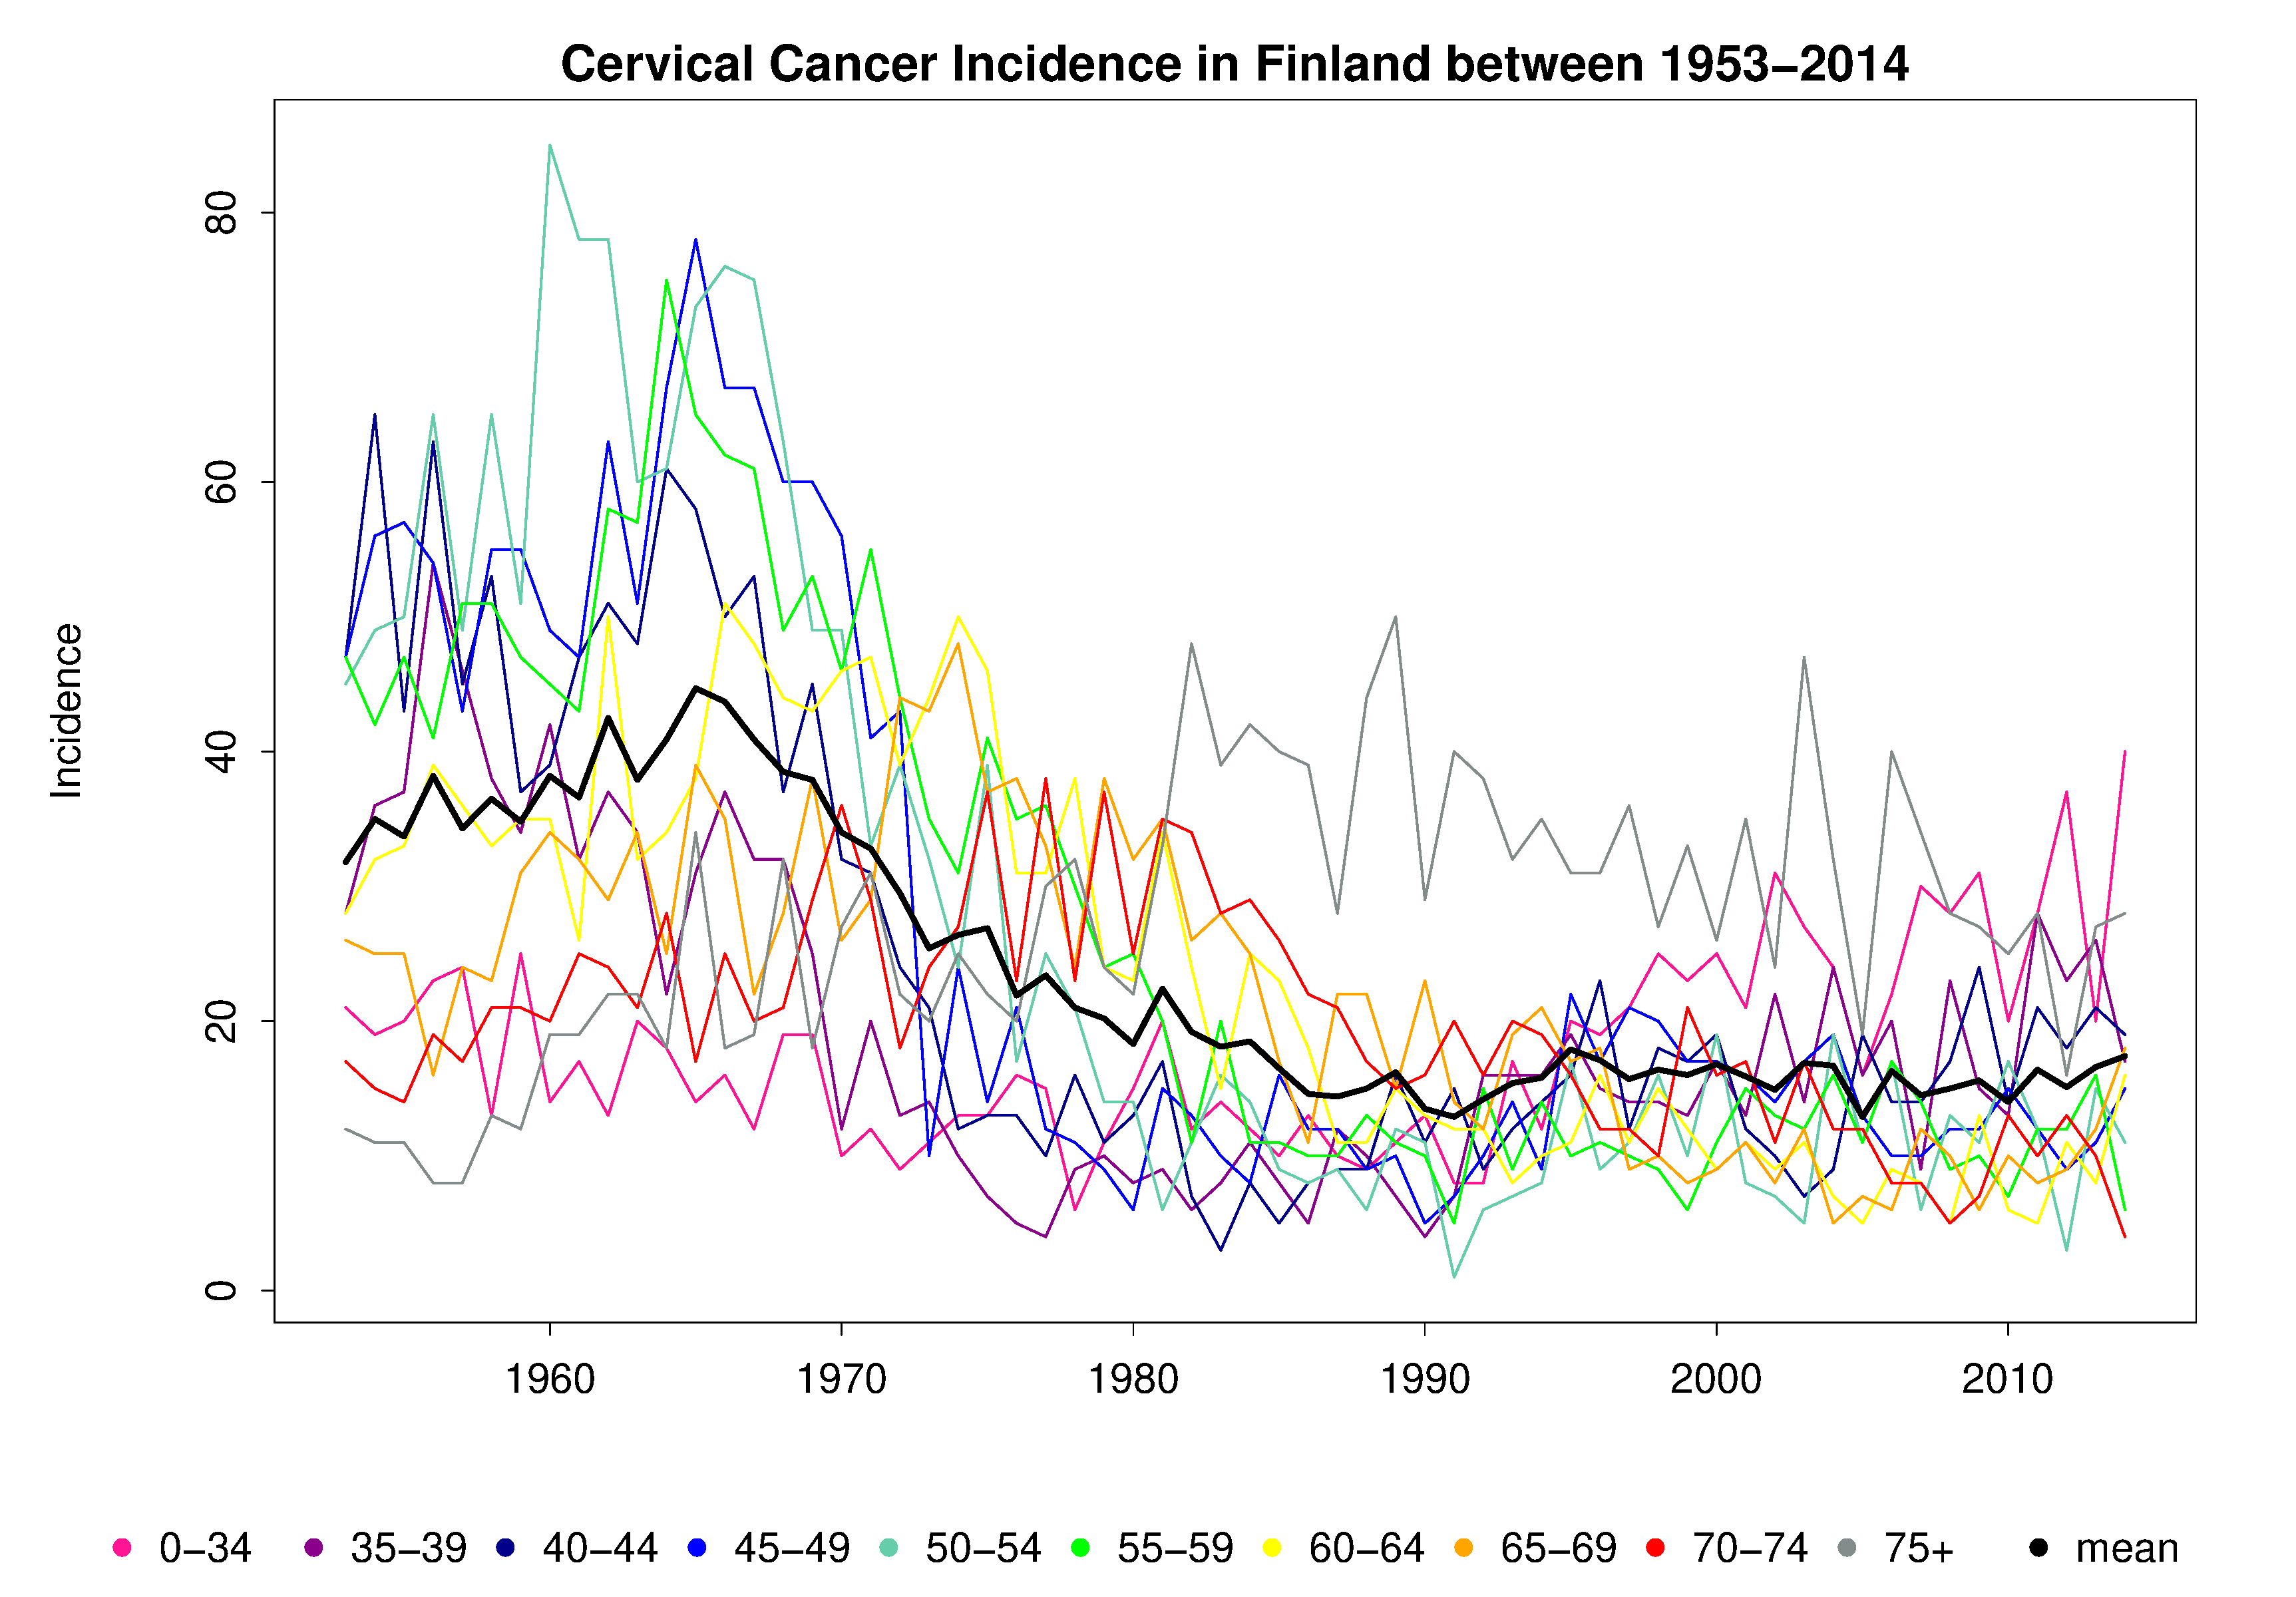
\includegraphics[width=1\linewidth]{cervicaloriginal.pdf}
\caption{Age stratified cervical cancer incidence in Finland between 1953 and 2014.}
\label{p1b}
\end{figure}

We performed the tICS transformation using the sample covariance matrix as the first scatter matrix and the sample autocovariance matrix with lag parameter $\tau=1$ as the second scatter matrix. 
The first three estimated tICS components are presented in Fig. \ref{tcomp}. We want to emphasize that the scales of the tICS components are not relevant. Instead, we seek for curves that have interesting shapes. The first three components have the largest corresponding absolute diagonal values on the estimated matrix $\Lambda$ and thus they are the most important. The remaining seven tICS components reveal no interesting structure and resemble noise. The remaining seven components are omitted from this paper.

 %First two components explain the trends seen in the original data very well.  
 
 
\begin{figure}
     \centering
     \subfloat[][First tICS comp]{ 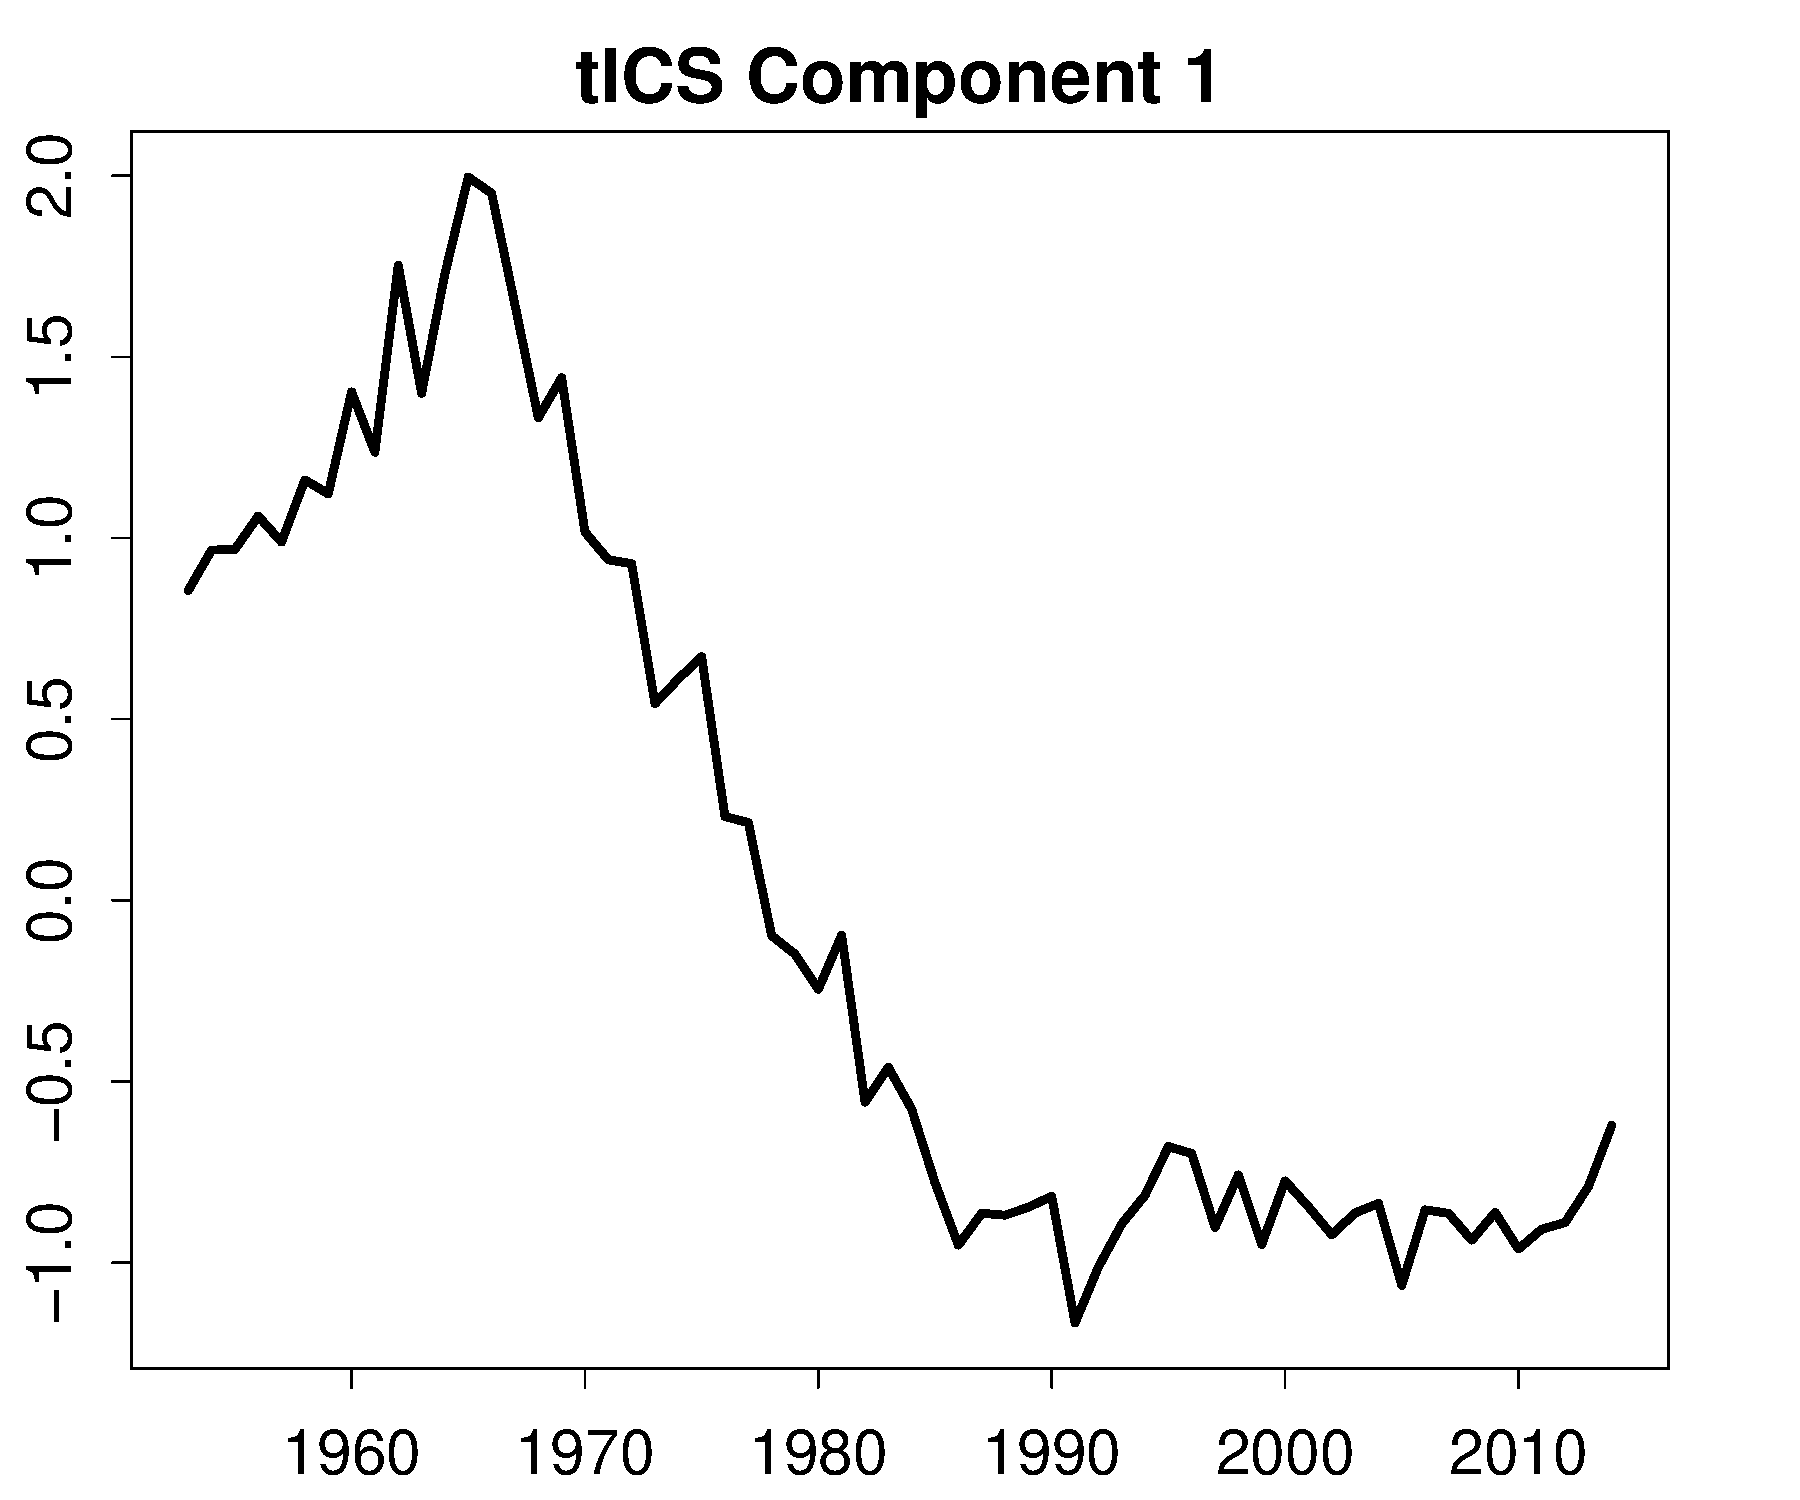
\includegraphics[width=0.33083\linewidth]{ccomp1.pdf}\label{cop1}}
     \subfloat[][Second tICS comp.]{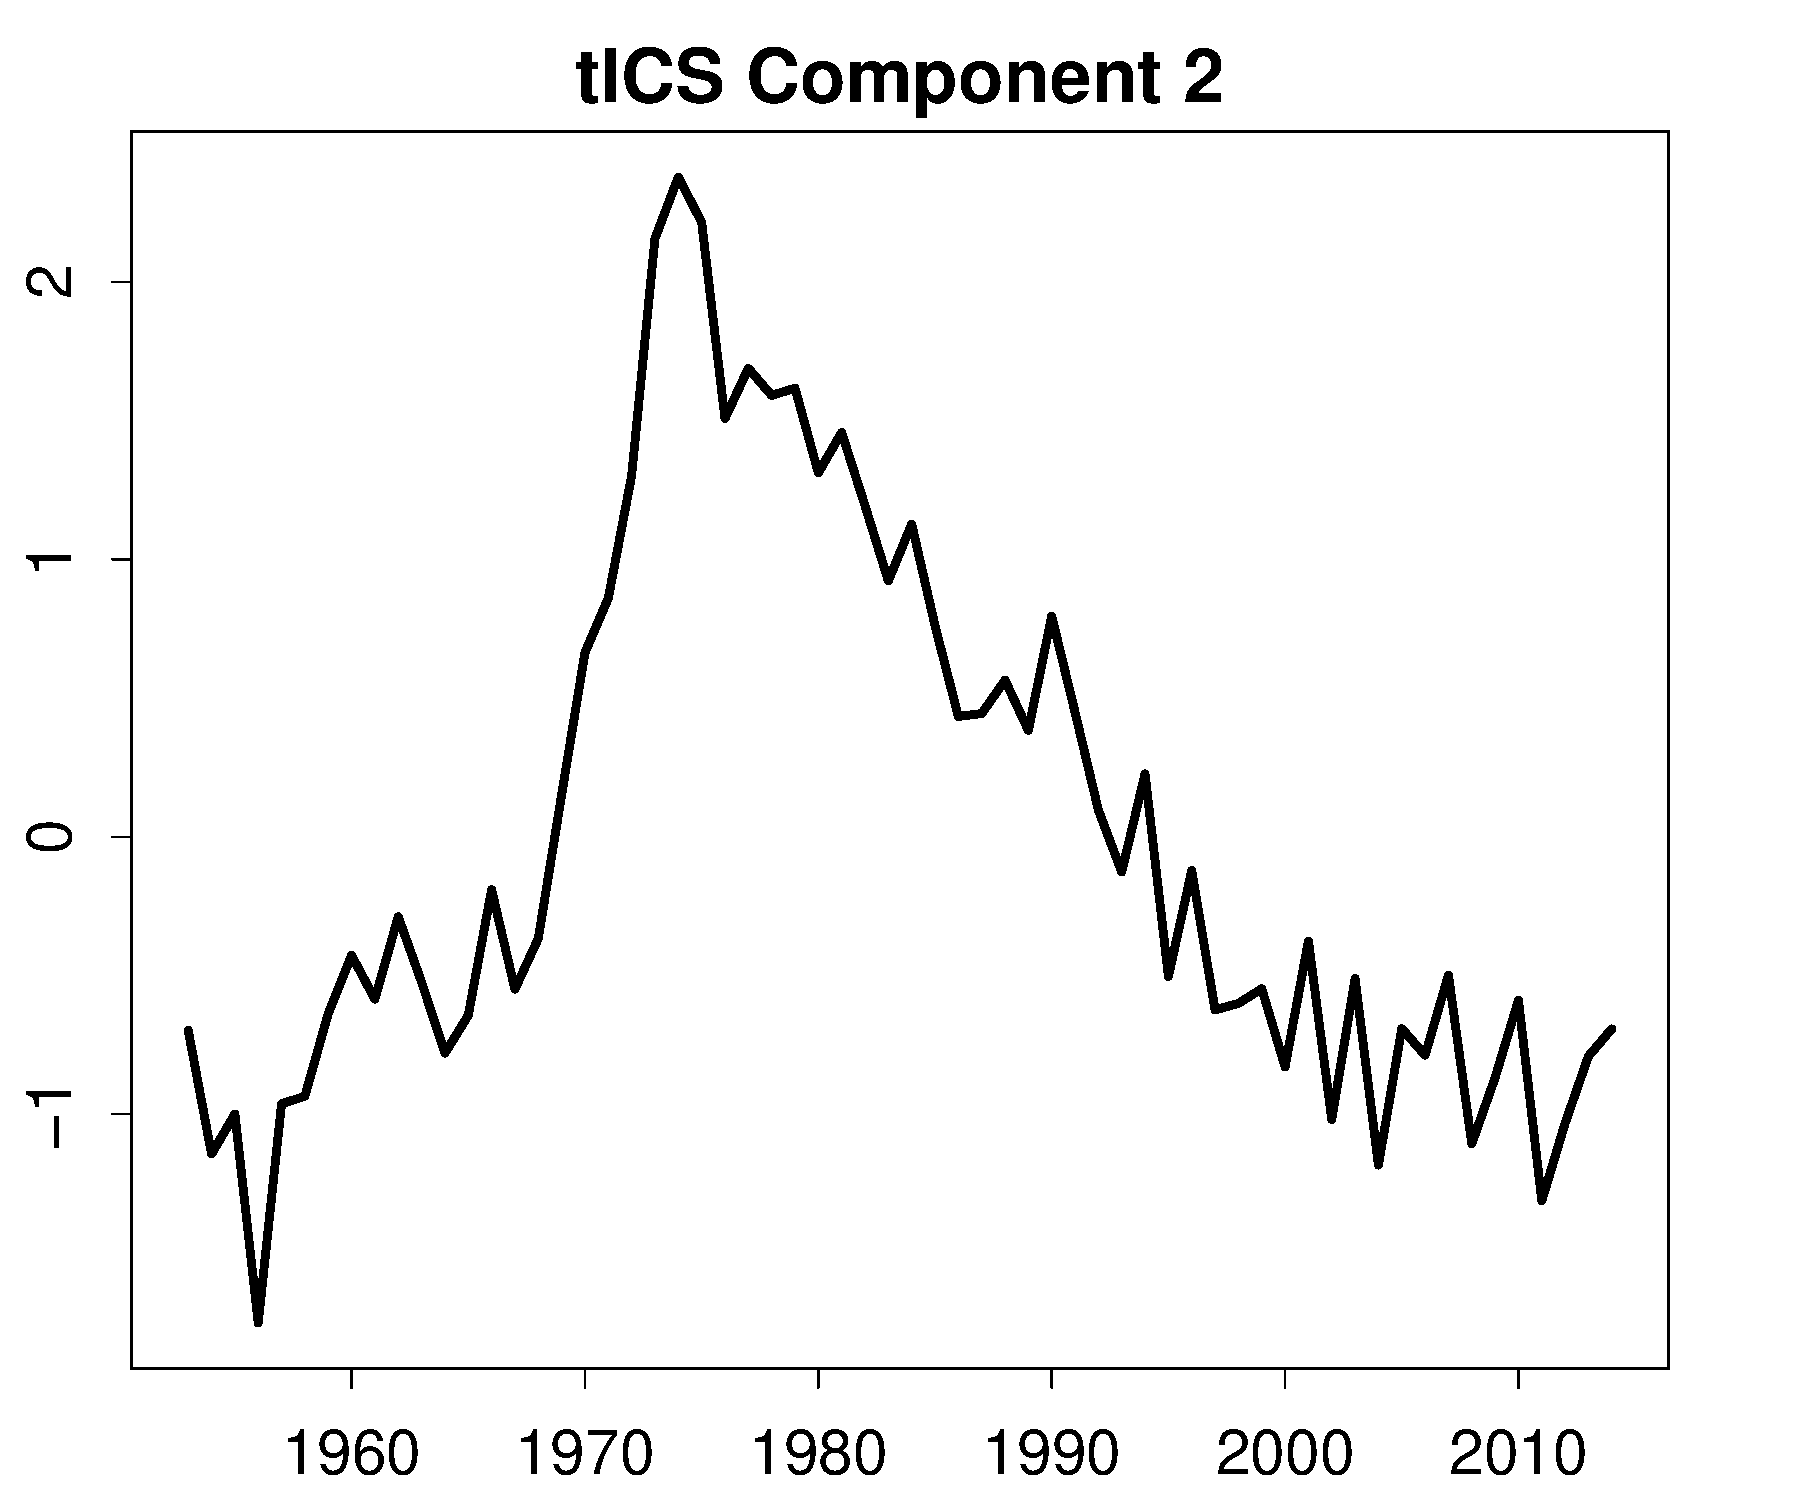
\includegraphics[width=0.33083\linewidth]{ccomp2.pdf}\label{p2}}
     \subfloat[][Third tICS comp.]{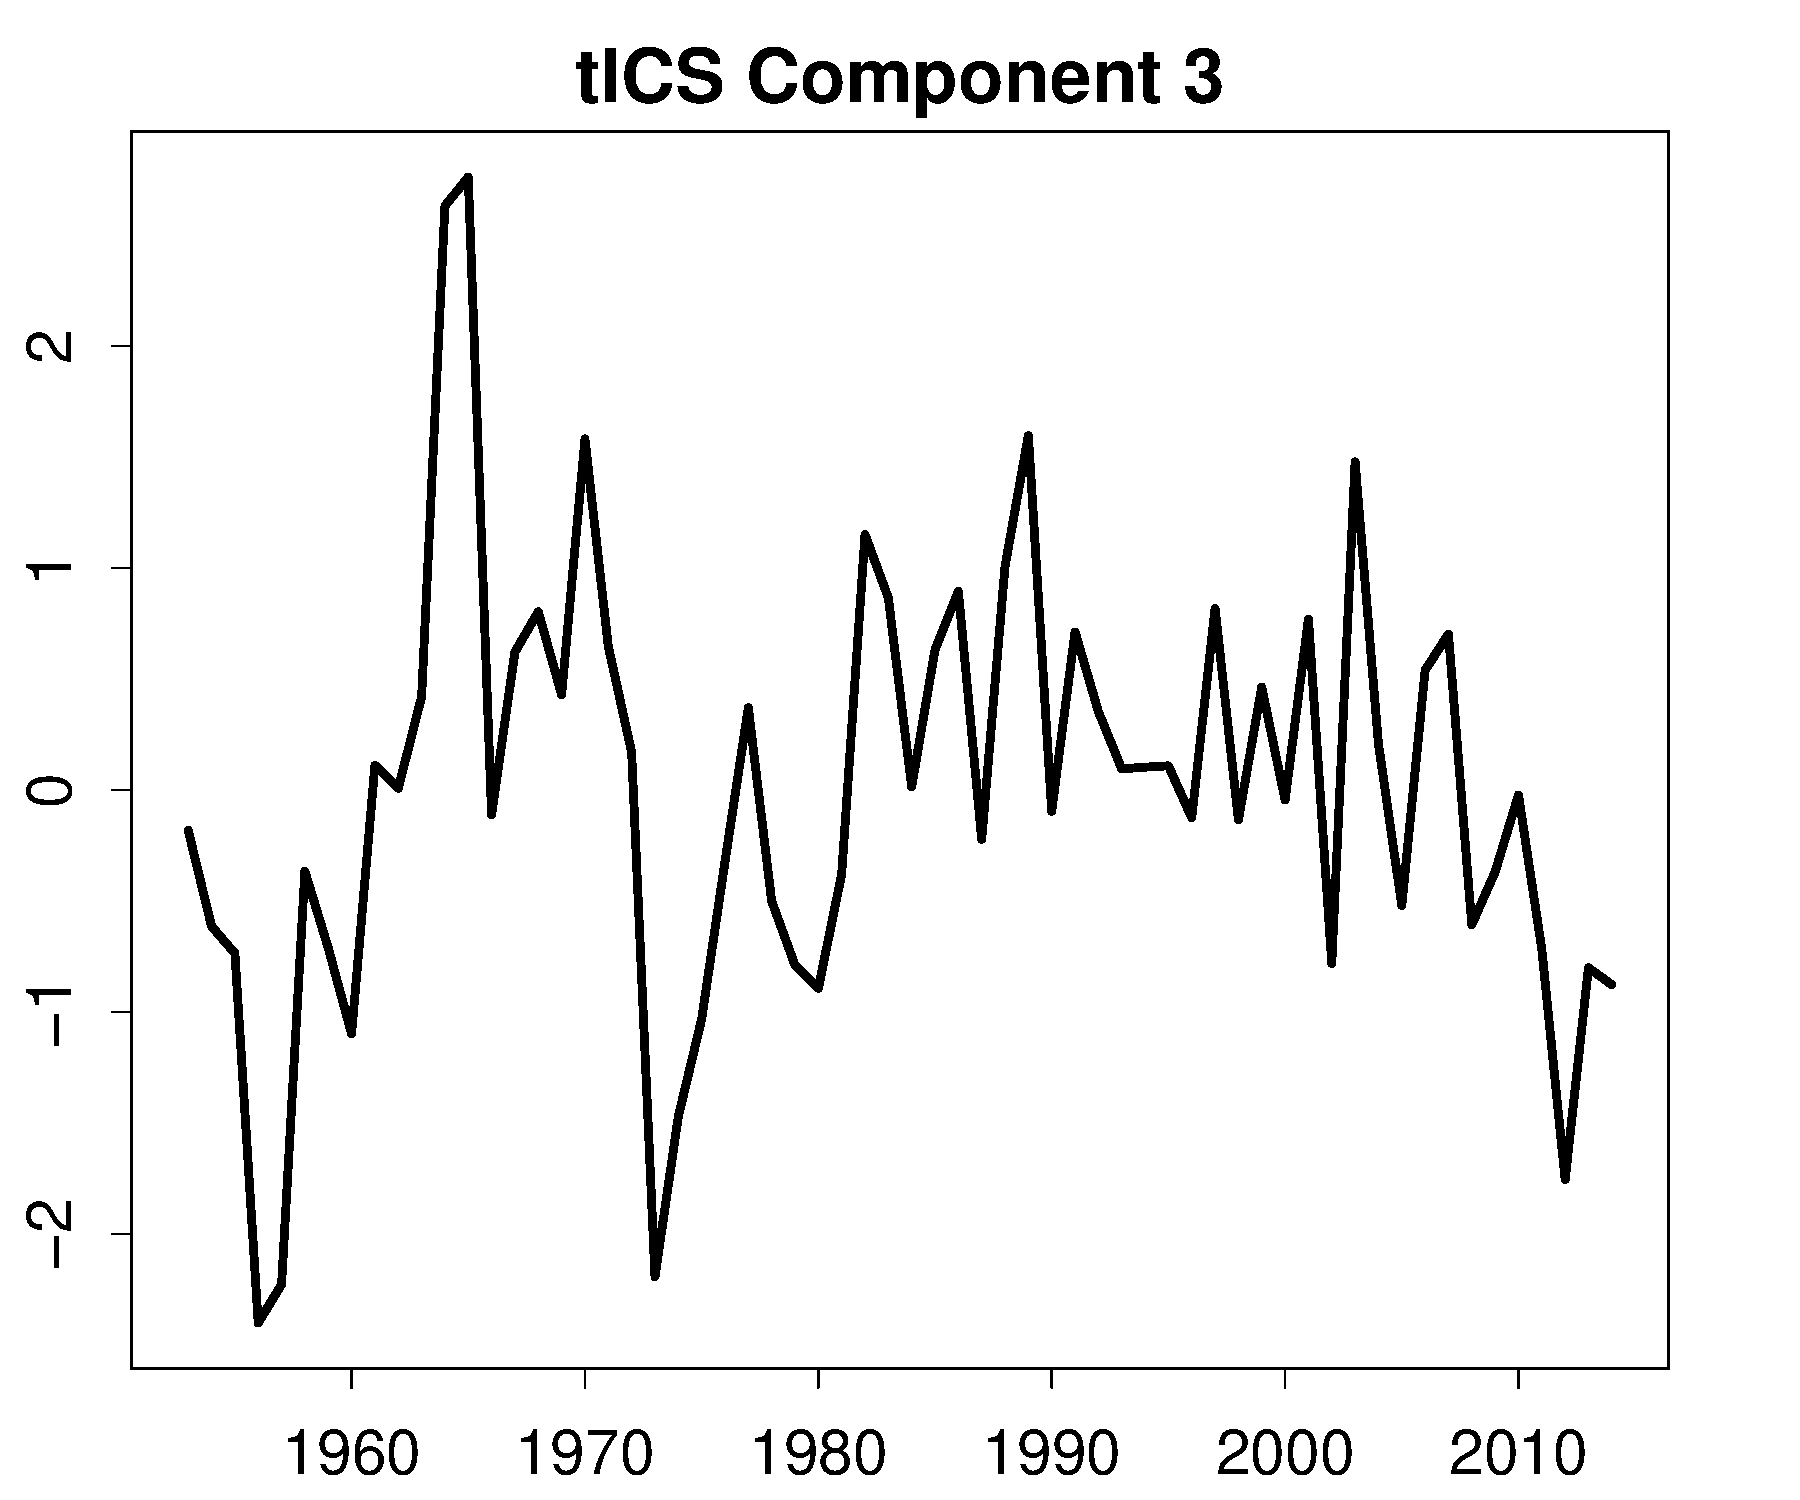
\includegraphics[width=0.33083\linewidth]{ccomp3.pdf}\label{cop3}}
     \caption{}
     \label{tcomp}
\end{figure}

 
The shape of the first component is similar to the mean curve time series, compare the black curve  in Fig. \ref{p1b} and the curve in Fig. \ref{cop1}. We name the first component as  ``the average''. The first component represents the average cervical cancel incidence.

The shape of the second tICS component is the most interesting, see Fig. \ref{p2}. It represents increasing trend from 1953 until mid--70s, and a decreasing trend after that. We call the second component ``the turning point". 

The third tICS component in Fig. \ref{cop3} is less interesting when compared to the first  tICS components. Like the last seven components, the third component  has a great deal of resemblance to random variation.




\begin{figure}
     \centering
 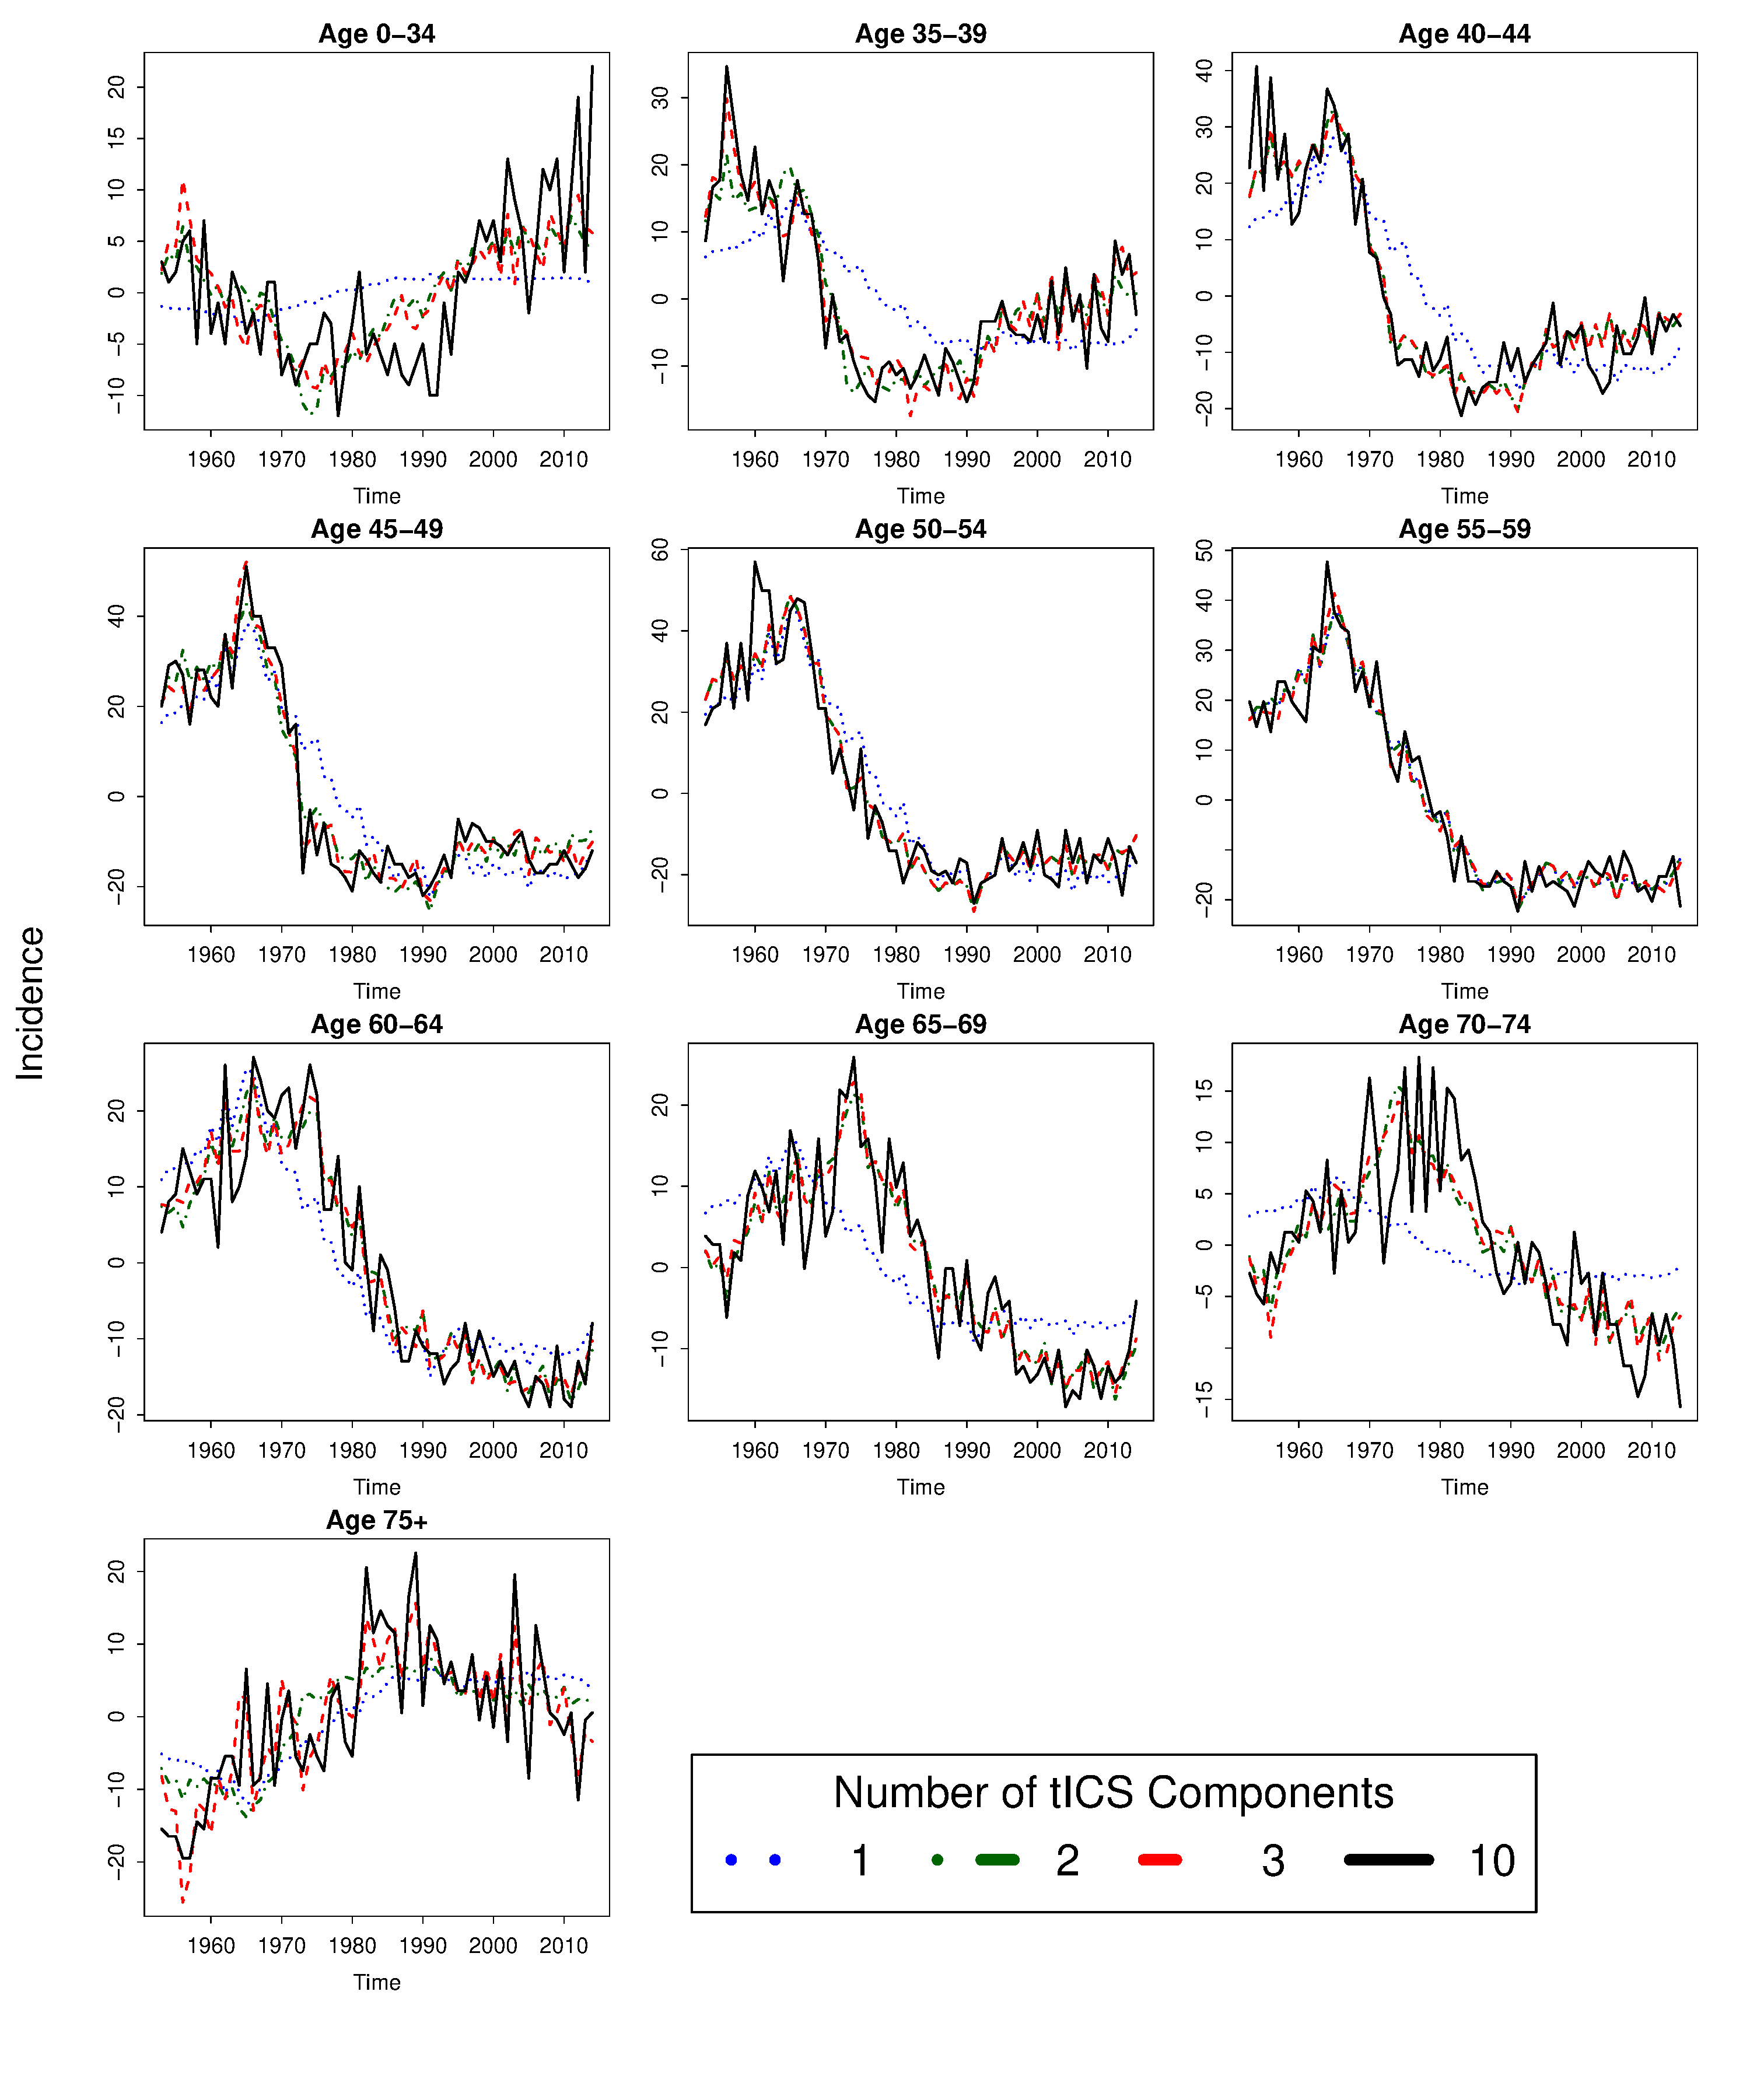
\includegraphics[width=1\linewidth]{dimticsfinal.pdf}
     
     %\subfloat{\includegraphics[width=0.90075\linewidth]{dimtics2.pdf}}


     \caption{Cervical cancer incidence in Finland between 1953 and 2014 in terms of estimated components. The estimation is performed using Eq. \ref{estimation}.}
     \label{dimred}
\end{figure}



The incidence curves in different age groups can be roughly estimated using only the first two components, see Eq. \ref{estimation} and  the green curves in Fig. \ref{dimred}. Most of the estimated incidence curves are relatively close to the observed curves. The age group of 0--34 has the least observations. Thus, random variation has a larger effect in this age group, which could be the reason for the estimate being worse when compared to the other age groups.






In order to visually observe cluster structures,  the scores of the components, i.e. the curves 
\begin{align*}
c_{ik} = \left[\hat{\Gamma}^{-1}\right]_{ik}z_t\left(k\right), \quad k\in\left\{1,2,3\right\}, \textnormal{ } i \in \left\{1,\ldots, p\right\},
\end{align*}
are presented in Fig. \ref{fig:cluster}, where $p=10$ is the number of age groups in our case study. We refer to the value $\left[\hat{\Gamma}^{-1}\right]_{ik}$ as the loading related to the age group $i$ and tICS component $k$. If the absolute value of the loading is large, that specific tICS component has a high impact in explaining the variation of the specific age group. The curves with the highest absolute loadings are the top and bottom curves in Fig. \ref{fig:cluster}. Likewise, low absolute loading values indicate that the specific tICS component has a low impact in explaining the variation of the specific age group. The curves with low absolute loadings are the middle curves in Fig. \ref{fig:cluster}.    The curves $c_{ik}$ provide visual clustering based on the first three components. 


\begin{figure}
     \centering
  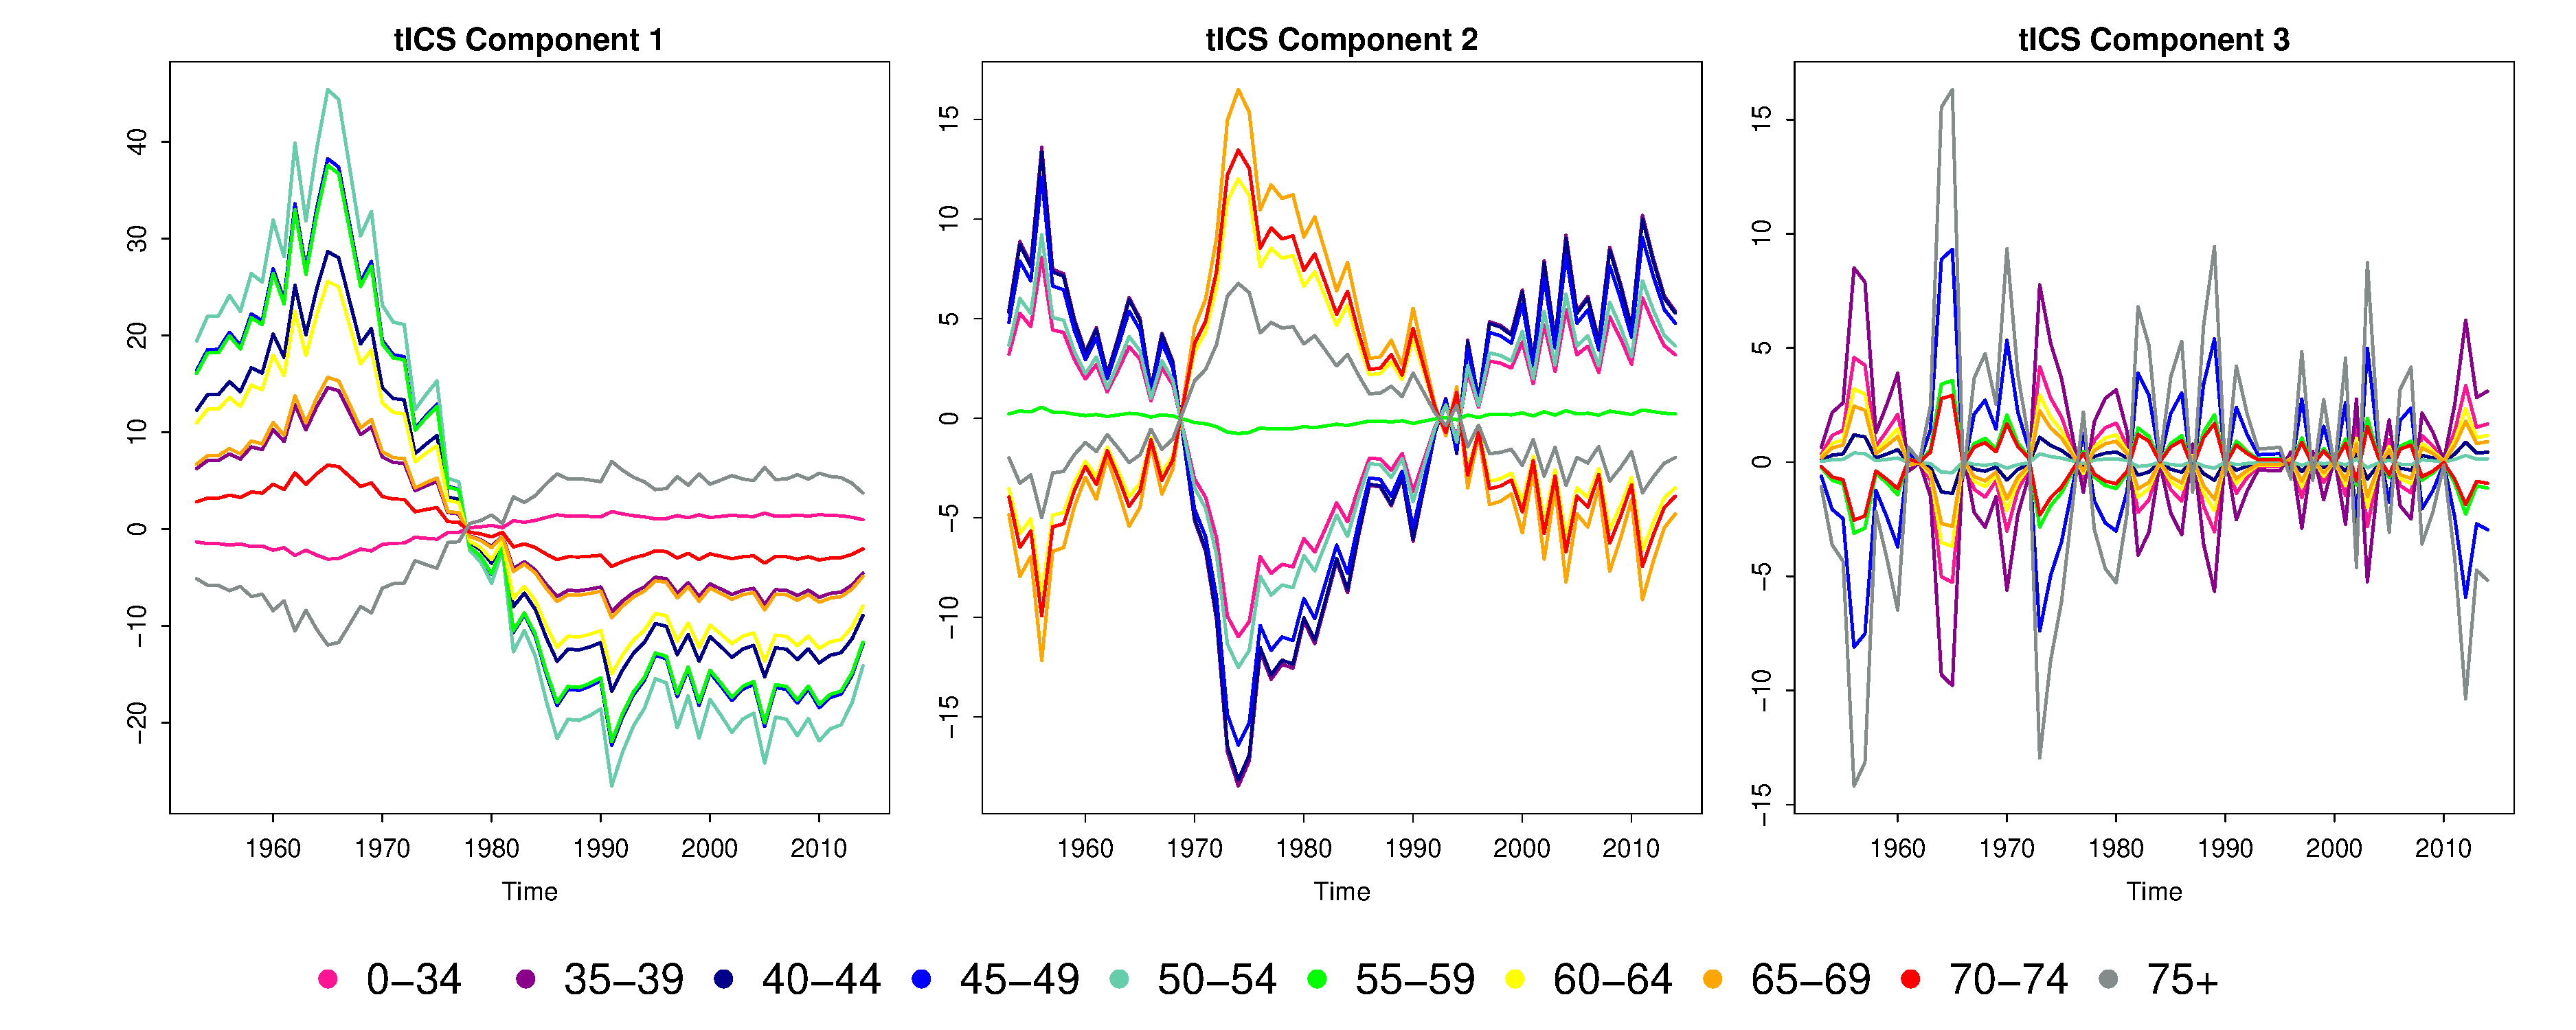
\includegraphics[width=1\linewidth]{clusteri.pdf}
     \caption{Clustered age stratified cervical cancer incidences for the first three tICS components. The curves are the tICS components multiplied with the corresponding loadings.}
     \label{fig:cluster}
\end{figure}



The first set of curves, $c_{\cdot 1}$, are ordered based on the trend of  cancer incidence in a specific age group. The curves representing age groups, where the incidence has been decreasing, i.e. the behavior is similar to the mean curve, have a positive loading in this component.  The largest positive loading is for the age group 50--54, which is the age group where the incidence has decreased the most. The age groups that have a negative loading with respect to the first component, have the first tICS component mirrored in Fig. \ref{fig:cluster}. The age group of  older than 75 has the largest negative loading with respect to the first component. The behavior of the incidence in this age group is the opposite compared to the mean cancer incidence, see Fig. \ref{p1b}.


The second set of curves, $c_{\cdot2}$, provide  clustering based on the second component in Fig. \ref{fig:cluster}. Visual clustering  reveals that the second component splits the age groups according to the age of menopause. Age groups of older than 60 have a positive loading, the age group of 55--59 has a loading close to zero and the age groups younger than 50 have a negative loading. 

Visual clustering based on the remaining components, including the third tICS component in Fig. \ref{fig:cluster}, reveal nothing interesting, as was expected from random variation.










\section{Discussion}\label{disc}

In our case study of cervical cancer incidence in Finland, tICS procedure produced interesting findings. 
The underlying structures  found by tICS procedure support recent findings discovered using other methods \cite{JP3}. The second tICS component was the most interesting one. The first component clustered the age groups with respect to trend. It separated the age groups where cancer incidence has been decreasing from those where the incidence  has been increasing or has stayed relatively same. The information provided by the clustering of the first component could also be easily be verified from Fig. \ref{p1b} and thus the clustering provided by this component is not particularly interesting. The components after the second one seemed to be random variation, i.e. uninteresting noise. The tICS components 4--10 were omitted from this paper for this reason.

The second tICS component clusters the age groups according to the approximate age of menopause. The behavior of this component supports the findings by Sepp\"{a} et al. \cite{JP3} of the calendar time varying contribution of early and late age related components in cervical cancer.  The first crossing point of the curves is soon after starting the cervical cancer screening. Hidden structures in the incidence in age groups close to menopause are different from those in the age groups far away from menopause. Thus, it seems that hormonal changes might have a significant role in etiology of cervical cancer. 


We performed the tICS procedure with several different lags parameters $\tau$, and the best separation was obtained using lag $\tau=1$. The corresponding lag produced the most distinct values for the diagonal elements of the estimated matrix $\Lambda$ and the best estimated curves in Fig. \ref{dimred}. However, the most interesting findings --- the cluster structures visible in Fig. \ref{fig:cluster} --- stayed almost identical with several different lags that were close to $\tau=1$. 

Furthermore, we applied the second order blind identification (SOBI) \cite{belouchrani1997} procedure for this data. In SOBI, the second diagonalization is replaced with a joint diagonalization with respect to multiple autocovariance matrices with distinct lags. This makes the choice of the lag parameter less decisive. The shapes of the first two components were similar to our findings. However, the first two SOBI components, with every set of lags that we tried, had considerably worse performance in explaining the variation using only two or three components, whereas the first two tICS components explain the variation of the original time series relatively well, see Fig. \ref{dimred}.



Since the  tICS procedure is affine invariant, it ensures that the findings are not simply artifacts of the used coordinate system. Exploratory tools such as PCA are not affine invariant.
Affine transformations of the original data would yield completely different results in PCA whereas tICS would remain unaffected. Furthermore, we applied the PCA transformation to this data set and the first two principal components were similar to the first two tICS components. However again, visual inspection of Fig. \ref{dimred} revealed that the first two and three principal components did not perform as well in estimating the original time series. 

In this paper, we  stratified the analysis according to age groups, but other types of stratifications are also possible. We could e.g. consider stratification according to cohort and for other cancer sites also to gender. In the Western countries we are facing increasing cancer burden \cite{parkin2011}. Risk factors of  specific cancer have been studied for a long time, and many of them have been established. Even then, attributable fraction to known risk factors is often quite low leaving us with the need of further understanding etiology of a studied cancer. Identification of latent components of cancer incidence may open new possibilities for this. Further, if age related latent components of cancer are modifiable, it is important for future efforts of reducing cancer burden in Finland. 





\bibliographystyle{abbrvnat}
\bibliography{na2}
\end{document}